\documentclass[12pt]{article}
\usepackage{latexsym,amsmath,amssymb,tabu,CJKutf8,bm,graphicx}
\usepackage{caption,float}
\usepackage{multirow,booktabs,diagbox}
\textwidth 6.5in \textheight 9in \oddsidemargin 0pt \topmargin -8pt
\pagestyle{plain}

\begin{document}
\begin{CJK}{UTF8}{gkai}
    \title{近日问题总结}
    \date{\today}
    \author{王鑫}
    \maketitle
    \section{花瓣网格:}
    初始网格结构为:\\        
    \begin{figure}[H]
     \centering
     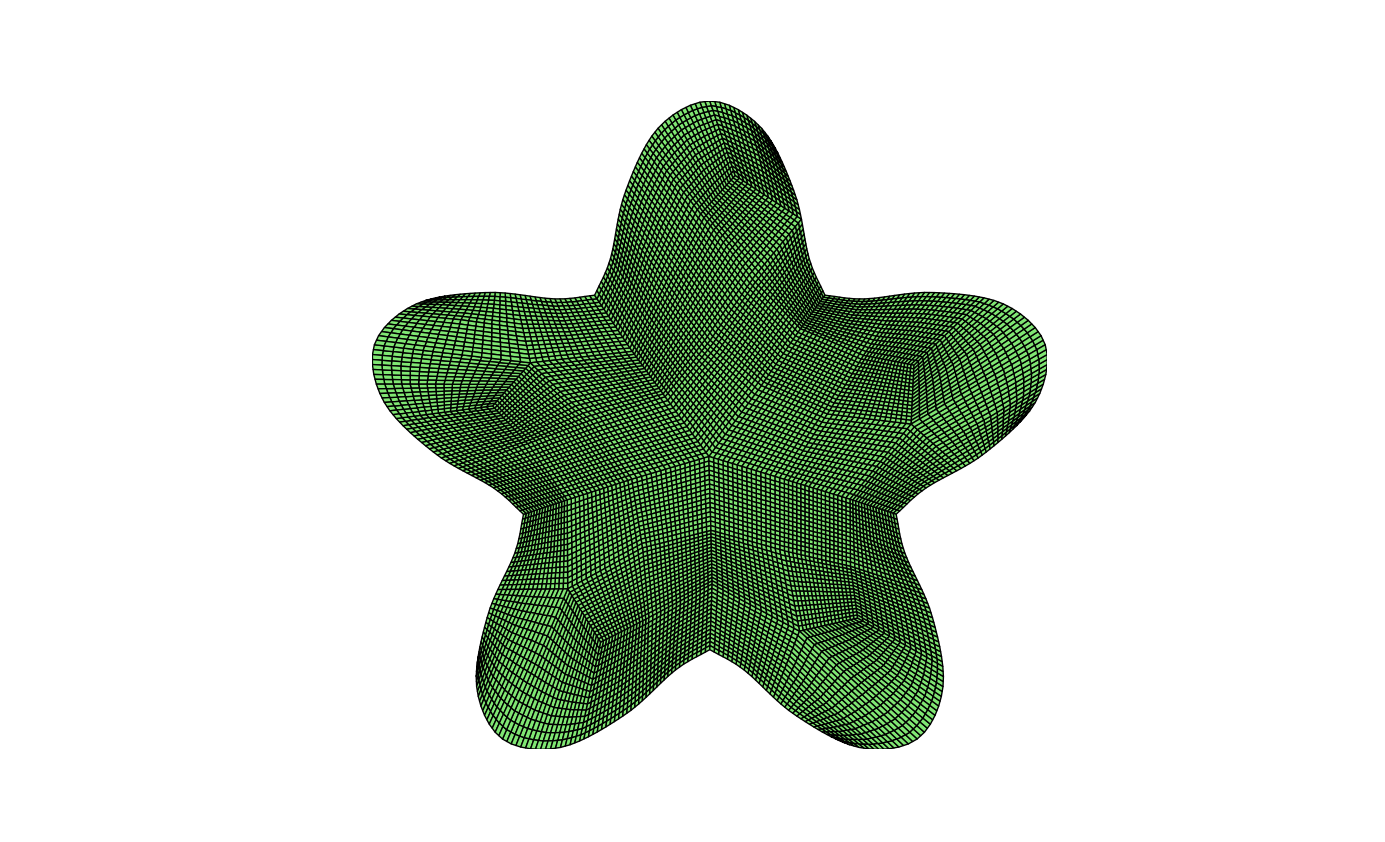
\includegraphics[width=8cm]{huaban1.png}
     \caption{}  		
     \end{figure}
当初值为六状相,即:\\
\begin{figure}[H]
	\centering
	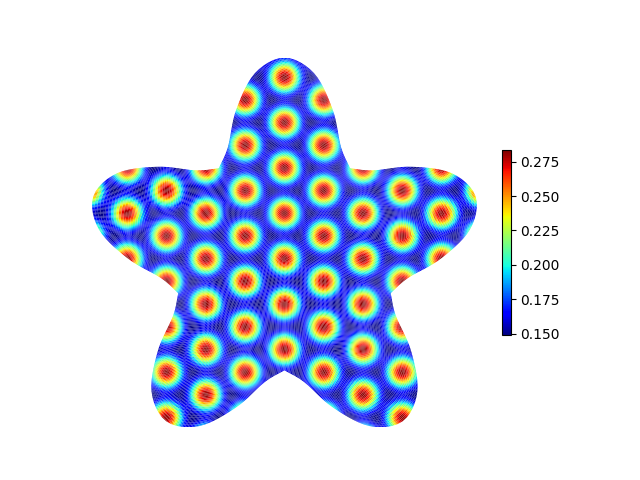
\includegraphics[width=8cm]{scftfigure0.png}
	\caption{}  		
\end{figure}
迭代22步得到的相结构为:\\

\begin{figure}[H]
	\centering   
	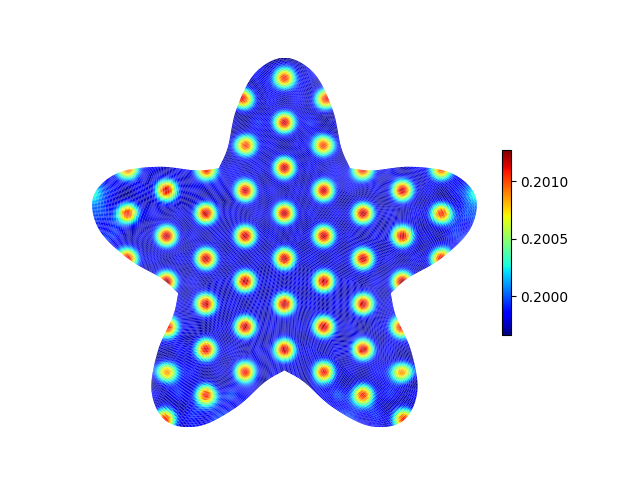
\includegraphics[width=8cm]{scftfigure22.png}
	\caption{}
\end{figure}
收敛时(迭代29步)的相结构为:\\
\begin{figure}[H]
	\centering   
	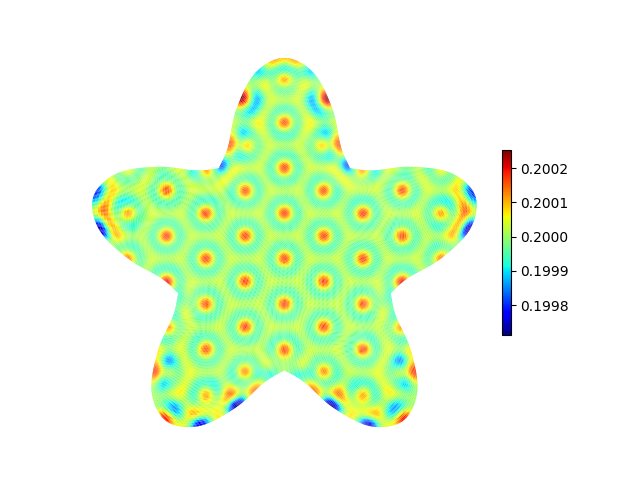
\includegraphics[width=8cm]{scftfigure28.png}
	\caption{}
\end{figure}   

我认为出现问题的地方:\\

1、第一步迭代的结果中H哈密顿量为正,且误差为-inf,数据结果如表\\
\begin{table}[H]
	\centering
\begin{tabular}{ccccc}
	\toprule
	区域$D/cm^2$ &	迭代步数 & Q&error &  H \\
	\midrule
	20*20&1& 6.572024684481041e-02 &-inf&4.119729499273764e+00 \\
	\bottomrule
\end{tabular}
\end{table}    
 
     
2、最终结果为均匀相,数据结果如下表:\\
\begin{table}[H]
	\centering
\begin{tabular}{ccccc}
	\toprule
	区域$D/cm^2$ &	迭代步数 & Q&error &  H \\
	\midrule
	20*20&29& 1.487861678781628e+01& 9.503887841155745e-07& -1.350116501325819e+00\\
	\bottomrule
\end{tabular}
\end{table}
当初值为层状相,即:\\
\begin{figure}[H]
	\centering
	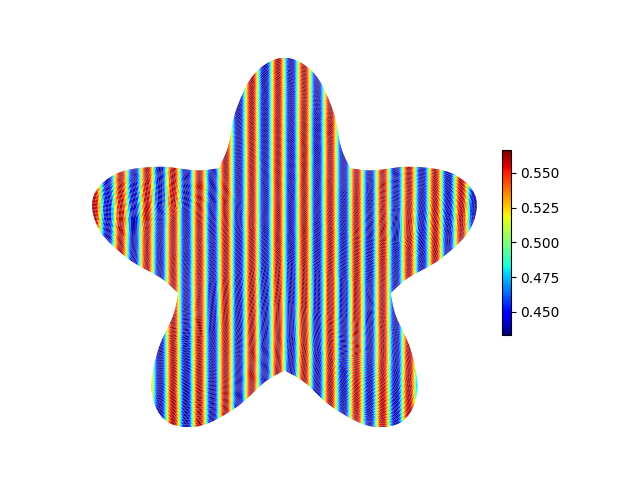
\includegraphics[width=8cm]{0.png}
	\caption{}  		
\end{figure}
迭代1480步的相结构为:\\
\begin{figure}[H]
	\centering   
	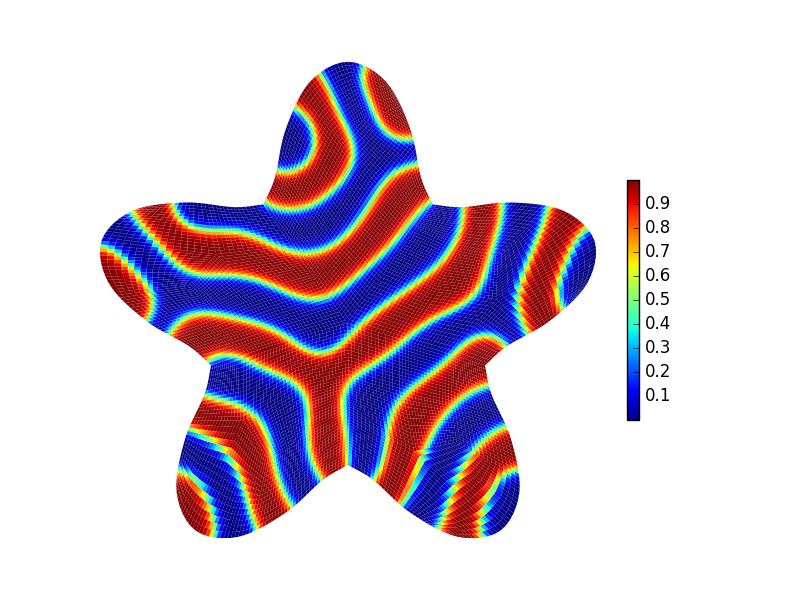
\includegraphics[width=8cm]{scftfigure1558.png}
	\caption{}
\end{figure}     
数据结果为:\\
\begin{table}[H]
	\centering
	\begin{tabular}{ccccc}
		\toprule
		区域$D/cm^2$ &	迭代步数 & Q&error &  H \\
		\midrule
		20*20&1480&3.110775692604836e+01& -1.078884831784421e-05& -1.772987671354151e+00 \\
		\bottomrule
	\end{tabular}
\end{table}    
问题所在:\\

  一直未达到收敛 \\ 
\section{海马网格}
    初始网格结构为:\\        
    \begin{figure}[H]
    	\centering
    	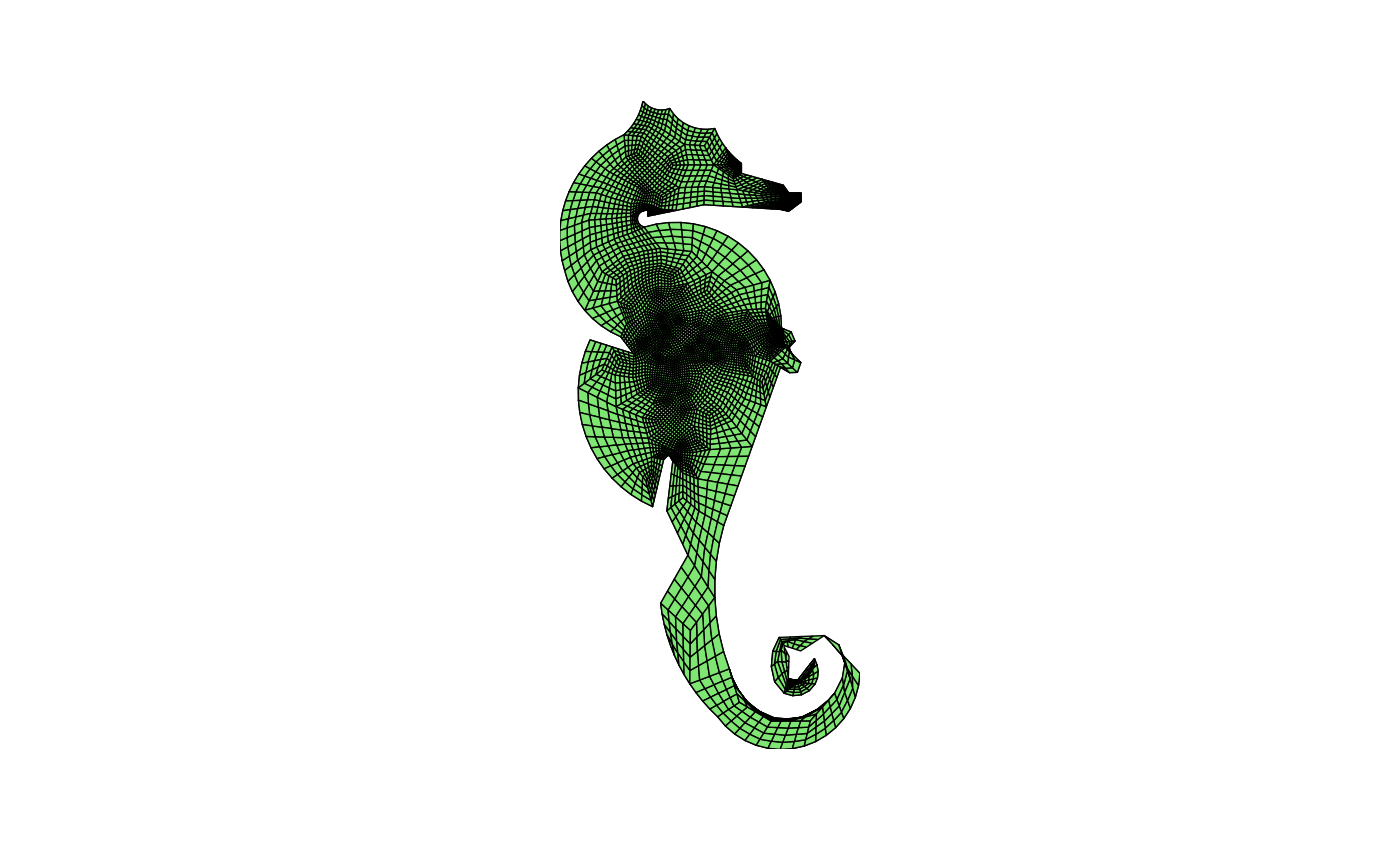
\includegraphics[width=8cm]{haima.png}
    	\caption{}  		
    \end{figure}    
\section{L型网格}
初始网格结构为:\\        
\begin{figure}[H]
	\centering
	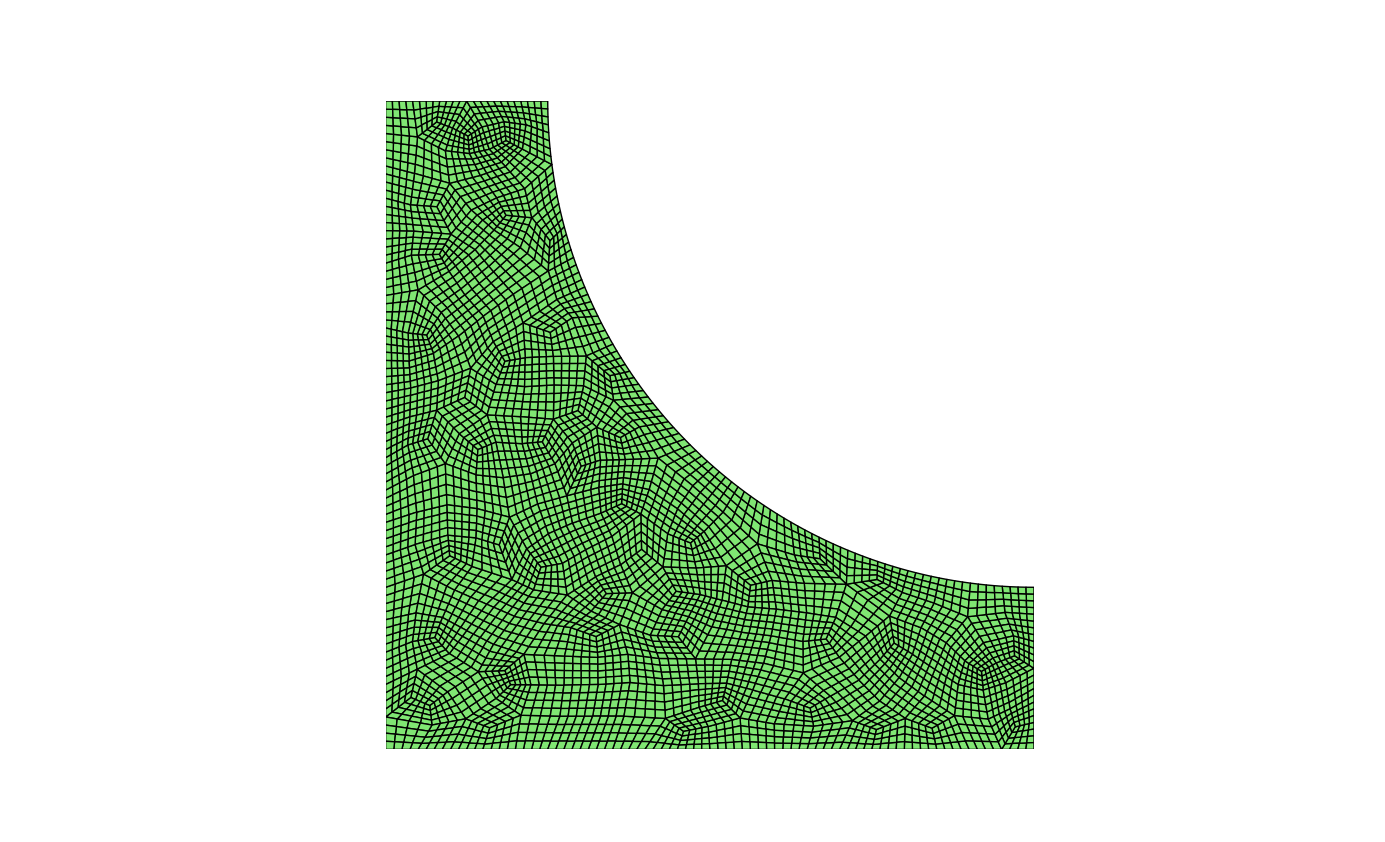
\includegraphics[width=8cm]{L.png}
	\caption{}  		
\end{figure}  
问题所在:\\

海马网格和L型网格数据读取成功,但是之后的程序过程有bug,具体见程序.\\  
\end{CJK}
\end{document}